\subsection{Proxy Re-Encryption}

\subsubsection{Introduction to Proxy Re-Encryption}

\begin{displayquote}{
  \textbf{"In a proxy re-encryption scheme a semi-trusted proxy converts a ciphertext for Alice into a ciphertext for Bob without seeing the underlying plaintext"}~\cite{greenateniese:2006:article}
}\end{displayquote}

Introduced as 'atomic proxy cryptography'~\cite{bbs:1998:book}, proxy re-encryption is the process of taking a message $M_a$, encrypted for a party $P_a$, and re-encrypting it such that it is readable by party $P_b$. Through the re-encryption process, the message is never decrypted by the proxy, such that the data is never revealed to any parties (including the proxy) other than the delegator and delegatees. This process relies on the functional relationship between the two ciphertexts, with the characteristics of the proxy re-encryption processed determined by the topology of this function.

\begin{figure}[H]
  \centering
  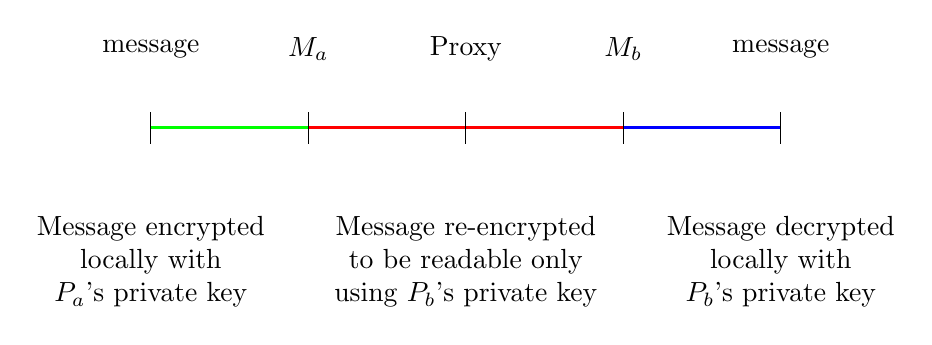
\begin{tikzpicture}

  \node at (0, 1)   {message} ;
  \node at (2, 1)   {$M_a$}   ;
  \node at (4, 1)   {Proxy}   ;
  \node at (6, 1)   {$M_b$}   ;
  \node at (8, 1)   {message} ;

  \draw [very thick, green] (0,0)   -- (2,0)   ;
  \draw [very thick, red]   (2,0)   -- (6,0)   ;
  \draw [very thick, blue]  (6,0)   -- (8,0)   ;
  \draw                     (0,-.2) -- (0, .2) ;
  \draw                     (2,-.2) -- (2, .2) ;
  \draw                     (4,-.2) -- (4, .2) ;
  \draw                     (6,-.2) -- (6, .2) ;
  \draw                     (8,-.2) -- (8, .2) ;

  \node[align=center, below] at (0, -1)%
    {Message encrypted\\locally with\\$P_a$'s private key};
  \node[align=center, below] at (4, -1)%
    {Message re-encrypted\\to be readable only\\using $P_b$'s private key};
  \node[align=center, below] at (8, -1)%
    {Message decrypted\\locally with\\$P_b$'s private key};

  \end{tikzpicture}
  \caption{
    Journey of a message using a proxy re-encryption scheme.
  }
\end{figure}


In figure \ref{fig:pre_example}, whether data is handled or manipulated by a fully trusted entity (a delegator or delegatee) or not is indicated using green/blue and red lines respectively.

The encrypted message $M_a$ is passed to the semi-trusted proxy along with the re-encryption key ( some $f(SK_a, PK_b)$\footnote{$SK_x$ represents the secret (private) key of a party $x$, $PK_x$ represents the public key of a party $x$.})

In the following sections I discuss the contributions of various authors through the history of proxy re-encryption and the available schemes that might be suitable for a project focused on providing secure data sharing and storage. Specific properties of different proxy re-encryption schemes are discussed first to aid in understanding the historical context of each paper.

\subsubsection{Properties of a proxy re-encryption scheme}

\begin{table}[H]
  \centering
  \begin{tabular}{ | l | c | c | c | }
    \hline
    Property & \cite{bbs:1998:book} & \cite{ivandodis:2003:inproceedings} & \cite{afgh:2006:article} \\
    \hline
    1. Unidirectional & & \checkmark & \checkmark \\
    2. Non-interactive & & \checkmark & \checkmark \\
    3. Proxy invisible & \checkmark & & \checkmark \\
    4. Original access & \checkmark & \checkmark & \checkmark \\
    5. Key optimal & \checkmark & & \checkmark \\
    6. Collusion 'safe' & & & \checkmark \\
    7. Temporary & \checkmark & \checkmark & \checkmark \\
    8. Non-transitive & & \checkmark & \checkmark \\
    9. Non-transferable & & & \\
    \hline
  \end{tabular}
  \caption{Comparison of properties of proxy re-encryption schemes}{
    \cite{afgh:2006:article} lists nine desirable properties of a proxy re-encryption scheme. Below is the table created by the author to show the benefits and compromises of the first three schemes discussed below.
  }
  \label{table:pre_properties}
\end{table}

\paragraph{Property Definitions}

\begin{enumerate}
  \item
    \textbf{Unidirectional} \\
    Creating a proxy key $\pi_{a \rightarrow b}$ allows re-encryption $A \rightarrow B$ but not $B \rightarrow A$.
  \item
    \textbf{Non-interactive} \\
    Re-encryption keys can be created with the public key from the delegatee, without the need for an authorised third party or any interaction.
  \item
    \textbf{Proxy invisible} \\
    It is not possible to determine that a proxy has re-encrypted a ciphertext. If a recipient receives a ciphertext that has been re-encrypted but is indistinguishable from a ciphertext which has only been encrypted by the recipient's public key, then the proxy has been invisible.
  \item
    \textbf{Original access} \\
    The delegator of some ciphertext retains the ability to decrypt ciphertexts that have been re-encrypted for a delegatee, thereby retaining the delegator's original access rights.
  \item
    \textbf{Key optimal} \\
    The storage of secret keys remains constant with every extra delegatee.
  \item
    \textbf{Collusion 'safe'} \\
    Should the proxy and the delegatees collude, they will be unable to reveal the secret key of the delegator.
  \item
    \textbf{Temporary} \\
    The delegatee is only able to decrypt messages encrypted by the delegator through a certain time period $i$.
  \item
    \textbf{Non-transitive} \\
    The proxy alone cannot re-delegate decryption rights, i.e. there does not exist a function $f(re_{a \rightarrow b}, re_{b \rightarrow c}) = re_{a \rightarrow c}$.
  \item
    \textbf{Non-transferable} \\
    Some proxy and delegatees are unable to re-delegate encryption rights, i.e. even with $re_{a \rightarrow b}, sk_b, pk_c$ one cannot share data with another party (a non-delegatee and not the delegator). This remains an open problem for proxy re-encryption.
\end{enumerate}

\subsubsection{Atomic Proxy Cryptography}

Recognising that it is intuitive to expect any good cryptography scheme to disallow any untrusted party to re-encrypt a ciphertext, \cite{bbs:1998:book} suggests that perhaps it is desirable to allow re-encryption of a ciphertext, but only for specific delegatees. This is subject to doing so atomically, i.e. without revealing the underlying plaintext, and without knowledge of the delegator or delegatee being exposed in the process. Conceptually this means that a delegator can encrypt once and have semi-trusted proxies re-encrypt for delegatees when desired.

Let's suppose we have a cryptography scheme whereby the following functions are observed:

\begin{itemize}
  \item $Gen(...)$: A generator of keys requiring arbitrary arguments
  \item $Encrypt(m, k)$: Allows the encryption of a message $m$ using key $k$ such that it is only decryptable by it's counterpart (or itself, if symmetric)
  \item $Decrypt(m, k)$: Allows the decryption of some encrypted message $m$ using the key $k$. Successful only if the message $m$ was encrypted (and intended for) the owner of the key $k$.
  \item $\Pi(m, rek_{a \rightarrow b})$: Allows the re-encryption of some encrypted message $m$ intended for the owner of key $a$ such that it is decryptable by the owner of key $b$.
  \item $ReGen(..., SK_a, PK_b)$: A generator of re-encryption keys requiring arbitrary arguments including keys required to decrypt
\end{itemize}

As an example, imagine you wished to share an image privately between several friends. You encrypt this image and generate re-encryption keys for your friends (delegatees). Publishing the image and the keys means any third party (including the friends themselves) are able to re-encrypt the encrypted image such that a delegatee is able to decrypt it and view it.

The importance of the re-encryption function being atomic cannot be understated. The re-encryption function $\Pi$ alters the ciphertext effectively performing $\Pi(m_a, RK_{a \rightarrow b}) = Encrypt(Decrypt(m_a, SK_a), PK_b)$. However, if $\Pi$ were not atomic, the decryption of the message $m_a$ would reveal the plaintext content of the message to the proxy.

The following trust axioms apply to proxy re-encryption (assuming perfect implementation). The latter axiom only applies to symmetric key cryptography. Since the latter axiom is an undesirable property, we seek to only use asymmetric (public-key) cryptography to maintain security (of both parties).

\begin{itemize}
  \item A (unconditionally) trusts B since B can decrypt on behalf of A
  \item B trusts A since A can calculate $SK_b$ using the proxy key and $SK_a$. (\textit{Symmetric keys only})
\end{itemize}

Given these properties, we will assume that asymmetric cryptography is a requirement of proxy re-encryption going forward.

\cite{bbs:1998:book} also discusses the notion of active versus passive proxy schemes distinguishing whether the delegatee has to cooperate or not in the creation of the proxy key. In practice, if the delegatee's public key is made available and is the only requirement from the delegatee then the delegator can delegate without the delegatee present, but otherwise, e.g. if the delegatee's secret key is required, the delegator needs the delegatee's cooperation to generate the proxy key required. Furthermore, in consideration of the delegator and delegatee's personally-identifying information, the proxy key can be distinguished as being transparent, translucent, or opaque depending on the ability of a third party to distinguish the two public keys the proxy is re-encrypting between.

\cite{bbs:1998:book} uses ElGamal encryption~\cite{elgamal:1985:article} as the basis for the proxy cryptography scheme suggested. A brief description of the protocol follows.

\paragraph{ElGamal Cryptography}

The ElGamal scheme includes the following functions:

\begin{itemize}
  \item $Gen(..., g, Z_n^*)$: A generator of keys requiring arbitrary arguments including some $g$, a generator in $Z_n^*$, itself a finite cyclic group of order $n$. Produces some secret key $\alpha$, whereby $0 \le \alpha \le n$, and a public key $g^\alpha$.
  \item $Encrypt(m, pk)$: Takes a random number, $r \in {0..n}$. Encrypts a message $m$ using the shared secret represented by $g^{ar} = k$, A's public key to some random power. Outputs the tuple $(g^r, mk \text{ mod } n)$.
  \item $Decrypt(<pk, c>, sk)$: Decrypts some encrypted message $c$ using the secret key $sk$. Successful only if the message $c$ was encrypted for the owner of the key $sk$.
\end{itemize}

It is based on the Diffie-Helman protocol and relies on the discrete logarithm problem of $A = g^a$ being difficult.

\paragraph{BBS Scheme}

Similar to the standard ElGamal scheme, the Blaze, Bleumer, Strauss (BBS) scheme uses the same parameters but uses them to different effect.

As part of key generation, we now take $n$ to be of the form $2q + 1$ with $n$ itself prime. The generator is taken as above, with the secret key $a$ in ${0..n - 1}$, i.e. relatively prime to $n$. The inverse is also required for this scheme, so $a^{-1} \text{ mod } 2q$ is also calculated. The public key (published) is calculated as $g^a \text{ mod } n$. Encryption and decryption differ slightly to the standard ElGamal scheme:

\begin{itemize}
  \item $Encrypt(m, pk)$: Takes a random number, $r \in Z_{2q}^*$. Encrypts a message $m$ using the shared secret represented by $g^r = k$, A's public key to some random power. Outputs the tuple $(pk^r \text{ mod } n, mg^r \text{ mod } n)$.
  \item $Decrypt(<pk, c>, sk_a)$: Decrypts some encrypted message $c$ using the secret key $sk_a$. Successful only if the message $c$ was encrypted for the owner of the key $sk_a$, A. Uses the inverse of the secret key to yield $(pk^r \text{ mod } n)^{a^{-1}} = g^r (\text{mod } n)$. Taking the inverse of this result, we have the decryption key for the ciphertext: $mg^r \text{ mod } n(g^r (\text{mod } n))^{-1} = m$
\end{itemize}

Noting that the actual message is encrypted with some random $r$, this acts as a symmetric key during the encryption / decryption process. When the public key of the recipient is raised by $r$, this yields a result which is only decryptable by the intended recipient. Therefore we need a (proxy) function which is able to achieve the following:

$$
\begin{aligned}
& f(pk_a^r \text{ mod } n, re_{a \rightarrow b}) & &=& pk_b^r \text{ mod } n \\
\implies & f((g^a)^r \text{ mod } n, re_{a \rightarrow b}) & &=& (g^b)^r \text{ mod } n \\
\implies & re_{a \rightarrow b} & &=& g^{a^{-1}} \times g^{b}
\end{aligned}
$$

Note that the re-encryption process is more efficient than the process of decrypting the data and then re-encrypting the data with another key, since only one, atomic, exponentiation is required.

Given the reencryption key shown above ($g^{a^{-1}} \times g^{b}$), bilateral trust is required. $A$ can learn $B$'s key and vice versa. This is not desirable for this project and so we must look for alternative schemes which do not have this issue.

\subsubsection{Proxy Cryptography Revisited}

\cite{ivandodis:2003:inproceedings} authored a scheme aiming to address some of the shortcomings of the original BBS scheme. Crucial improvements include the scheme being unidirectional and non-transitive. However, the scheme does not allow true re-encryption as the delegatee is unable to decrypt the re-encryption with their self-generated private key.

\begin{itemize}
  \item $Gen(...)$: A generator of keys requiring arbitrary arguments
  \item $Encrypt(m, k)$: Allows the encryption of a message $m$ using key $k$ such that it is only decryptable by it's counterpart (or itself, if symmetric)
  \item $Decrypt(m, k)$: Allows the decryption of some encrypted message $m$ using the key $k$. Successful only if the message $m$ was encrypted (and intended for) the owner of the key $k$.
  \item $ReGen(..., SK_a)$: A generator of re-encryption keys requiring arbitrary arguments including the secret key of the delegator
\end{itemize}

Whilst the Ivan-Dodis (ID) scheme adds uni-directionality and non-transitivity to the original BBS scheme, it does so by compromising the very principle of re-encryption. \cite{ivandodis:2003:inproceedings} presents a generic scheme that can be applied to any asymmetric cryptography scheme. This is possible by allowing the key generation, encryption, and decryption algorithms to be the same as the underlying cryptography scheme. The algorithm to generate re-encryption keys relies on the idea that the private key, corresponding to the public key that was used to encrypt the data, can be split into two secrets. It is suggested by the author that the scheme is compatible with identity-based cryptography, RSA cryptography, and ElGamal cryptography. However, the practical use of RSA would require an algorithm for prime factorisation which does not exist for classical computers. Identity-based cryptography would rely on the use of a centralised identity provider and is therefore irrelevant to this project.

Furthermore, the two secrets composing the private key do not facilitate true re-encryption nor allow the delegatee to use their own self-generated key pair. The re-encryption process relies on the proxy to first decrypt the encryption using the first secret, and the delegatee is expected to use the second secret to perform a second decryption, i.e. $\text{Dec}_2(\text{Dec}_1(\text{Enc}, \text{secret}_1), \text{secret}_2) = m$. Clearly this is not collusion-safe and would forbid the publication of re-encryption keys.

\subsubsection{Improved Proxy Re-encryption Schemes with Applications to Secure Distributed Storage}

The proxy re-encryption scheme (AFGH) presented by \cite{afgh:2006:article} offers another take on proxy re-encryption, and is founded upon comparing previous schemes and offering improvements. The AFGH scheme offers all benefits of both previously discussed schemes (BBS and ID) as well as the option of a collusion 'safe' protocol.

One crucial problem with the scheme presented by \cite{ivandodis:2003:inproceedings} is that it does not yield proxy re-encryption as described. By splitting the private key as shares, apart from the obvious security issues, the delegatee is unable to decrypt the re-encrypted ciphertext with their own private key. Furthermore, the space requirement of two key shares per delegation in a system designed to scale is troubling.

Having attempted to improve the ID scheme by suggesting ways to split the secret keys and secure these to facilitate pseudo proxy re-encryption, the (AFGH) scheme authored by \cite{afgh:2006:article} uses an improved BBS scheme with bilinear maps allowing re-encrypted ciphertexts to be decrypted using a delegatees's normal secret key and improving upon the security of both the BBS and ID schemes.

The paper presents two useful schemes which differ only slightly. As the author states, the schemes operate using the BBS scheme over two groups $G_1, G_2$ of prime order $q$ with a bilinear map $e : G_1 \times G_1 \rightarrow G_2$. The system then uses $g$ a random generator in $G_1$, and $Z = e(g, g) \in G_2$.

First-level encryption refers to encrypting with the public key of A such that only A can decrypt the ciphertext, using $sk_a$. Second-level encryption refers to encrypting with the public key of A such that both A and their delegatees are able to decrypt the ciphertext.

\begin{itemize}
  \item
    \textbf{Key Generation} \\
    1. Produces a user's key pair of the form $(sk_a, pk_a) = (a, g^a)$. \\
    2. Produces a user's key pair of the form $(sk_a, pk_a) = ((a_1, a_2), (Z^{a_1}, g^{a_2}))$.
  \item
    \textbf{Re-encryption Key Generation} \\
    1. For a delegatee B, A publishes $re_{a \rightarrow b} = g^{\frac{b}{a}}$ using B's public key. \\
    2. For a delegatee B, A publishes $re_{a \rightarrow b} = g^{a_1 b_2}$ using B's public key.
  \item
    \textbf{First-level Encryption} \\
    1. Encrypt a message m $\in G_2$ using $pk_a$. Outputs $(Z^{ak}, mZ^{k})$. \\
    2. Encrypt a message m $\in G_2$ using $pk_a$. Outputs $c_{a, 1} = (Z^{a_1 k}, mZ^{k})$ ($c_{a, 2} = (Z^{a_2 k}, mZ^{k})$ for proxy invisibility).
  \item
    \textbf{Second-level Encryption} \\
    1. Encrypt a message m $\in G_2$ using $pk_a$. Outputs $(g^{ak}, mZ^{k})$. \\
    2. Encrypt a message m $\in G_2$ using $pk_a$. Outputs $(g^k, mZ^{a_1 k})$.
  \item
    \textbf{Re-encryption} \\
    1. Using $re_{a \rightarrow b}, (g^{ak}, mZ^{k})$ (i.e. a second-level encryption), compute $Z^{bk} = e(g^{ak}, g^{\frac{b}{a}})$. Outputs $(Z^{bk}, mZ^{k})$ (i.e. a first-level encryption). \\
    2. Using $re_{a \rightarrow b}, (g^k, mZ^{a_1 k})$ (i.e. a second-level encryption), compute $Z^{b_2 a_1 k} = e(g^k, g^{a_1 b_2})$. Outputs $(Z^{b_2 a_1 k}, mZ^{a_1 k}) = (Z^{b_2 k'}, mZ^{k'})$ (i.e. a first-level encryption).
  \item
    \textbf{Decryption (using first-level encryption)} \\
    1. Given $c_a = (\alpha, \beta)$, compute $m = \frac{\beta}{\alpha^{\frac{1}{a}}}$. \\
    2. Given $c_{a, i} = (\alpha, \beta)$, compute $m = \frac{\beta}{\alpha^{\frac{1}{a_i}}}$.
  \item
    \textbf{Decryption (using second-level encryption)} \\
    1. Given $c_a = (\alpha, \beta)$, compute $m = \frac{\beta}{e(\alpha, g)^{\frac{1}{a}}}$. \\
    2. Given $c_a = (\alpha, \beta)$, compute $m = \frac{\beta}{e(\alpha, g)^{a_1}}$.
\end{itemize}

In terms of the proxy re-encryption properties discussed above, both schemes fair well. The former scheme is unidirectional, non-interactive, proxy invisible, collusion safe, key optimal, and non-transitive. The main difference in the two schemes is that the latter replaces the use of a single secret key with dual secret keys, such that encryptions intended to be kept private and those with delegatees are strictly separate. This scheme therefore requires fewer assumptions to be proved secure.

% \subsubsection{Unidirectional Chosen-Ciphertext Secure Proxy Re-Encryption}

% \cite{lv11:2011:article}

\subsubsection{Post-Quantum Cryptography}

An area of rising concern for cryptography is that of a post-quantum world. Whilst not a key consideration for this project, it highlights the need to make software and architecture that is adaptable and flexible to its own vulnerability. Post-quantum cryptography largely concerns the use of Shor's algorithm (public key cryptography) and Grover's algorithm (symmetric key cryptography) on a quantum computer to solve problems that are intractable on non-quantum computers. A brief summary of how post-quantum cryptography affects proxy re-encryption follows.

\cite{shor:1999:article} authored an algorithm to do prime factorisation and challenge the discrete logarithm problem. Since proxy re-encryption requires an asymmetric cryptography scheme to function, such an algorithm threatens its future security. The RSA and ElGamal schemes use prime factorisation and the discrete logarithm problem respectively as their key security features. Therefore, neither of these schemes will be secure against attacks from a large-enough (sufficient qubits) quantum computer.

Not directly used in proxy re-encryption, but often as a consequence of encrypting binary data, symmetric cryptography is similarly (although less effectively) compromised by an algorithm authored by \cite{grover:1996:inproceedings}. It is widely thought that using Grover's algorithm a symmetric cryptography scheme (such as AES) would have security equal to that of half it's key length when challenged by a quantum computer. Therefore, the use of a 256-bit key would imply that the encryption is safe up to the security of a 128-bit key on a classical computer.
